%===============================================================================
% VESTA RISC-V Core Block Diagram
% A clean, professional block diagram for presentations
%===============================================================================

\documentclass[tikz, border=10pt]{standalone}
\usepackage{tikz}
\usetikzlibrary{shapes.geometric, arrows.meta, positioning, fit, calc, backgrounds, shadows}

%-------------------------------------------------------------------------------
% Color Definitions - Professional color palette
%-------------------------------------------------------------------------------
\definecolor{cpuCore}{RGB}{70, 130, 180}        % Steel blue - main core
\definecolor{controlUnit}{RGB}{255, 140, 66}    % Orange - control
\definecolor{dataUnit}{RGB}{100, 180, 100}      % Green - datapath
\definecolor{memoryUnit}{RGB}{140, 100, 180}    % Purple - memory/CSR
\definecolor{irqUnit}{RGB}{220, 80, 80}         % Red - interrupts
\definecolor{sramColor}{RGB}{80, 80, 120}       % Dark blue-gray - SRAM
\definecolor{textLight}{RGB}{255, 255, 255}     % White text
\definecolor{borderDark}{RGB}{40, 40, 40}       % Dark borders
\definecolor{bgLight}{RGB}{250, 250, 250}       % Light background
\definecolor{signalLine}{RGB}{60, 60, 60}       % Signal lines

%-------------------------------------------------------------------------------
% TikZ Styles
%-------------------------------------------------------------------------------
\tikzstyle{mainblock} = [
    rectangle, 
    rounded corners=8pt,
    minimum width=3.5cm, 
    minimum height=1.2cm,
    text centered, 
    draw=borderDark, 
    line width=1.5pt,
    font=\bfseries\sffamily,
    text=textLight,
    drop shadow={shadow xshift=2pt, shadow yshift=-2pt, opacity=0.3}
]

\tikzstyle{subblock} = [
    rectangle, 
    rounded corners=4pt,
    minimum width=2cm, 
    minimum height=0.8cm,
    text centered, 
    draw=borderDark, 
    line width=1pt,
    font=\small\sffamily,
    text=textLight
]

\tikzstyle{tinyblock} = [
    rectangle, 
    rounded corners=3pt,
    minimum width=1.4cm, 
    minimum height=0.55cm,
    text centered, 
    draw=borderDark!70, 
    line width=0.8pt,
    font=\scriptsize\sffamily,
    text=textLight
]

\tikzstyle{memblock} = [
    rectangle, 
    rounded corners=6pt,
    minimum width=2.8cm, 
    minimum height=1.8cm,
    text centered, 
    draw=borderDark, 
    line width=1.5pt,
    font=\bfseries\sffamily,
    text=textLight,
    drop shadow={shadow xshift=2pt, shadow yshift=-2pt, opacity=0.3}
]

\tikzstyle{ioport} = [
    rectangle,
    rounded corners=2pt,
    minimum width=2cm,
    minimum height=0.55cm,
    text centered,
    draw=borderDark,
    line width=1pt,
    font=\small\sffamily\bfseries,
    fill=white,
    text=borderDark
]

\tikzstyle{signal} = [
    -{Stealth[length=3mm, width=2mm]},
    line width=1.2pt,
    color=signalLine
]

\tikzstyle{bussignal} = [
    -{Stealth[length=3mm, width=2mm]},
    line width=2.5pt,
    color=signalLine
]

\tikzstyle{bidirectional} = [
    {Stealth[length=2.5mm, width=1.8mm]}-{Stealth[length=2.5mm, width=1.8mm]},
    line width=1.2pt,
    color=signalLine
]

\tikzstyle{databidirectional} = [
    {Stealth[length=3mm, width=2mm]}-{Stealth[length=3mm, width=2mm]},
    line width=2.5pt,
    color=signalLine
]

\tikzstyle{containerbox} = [
    rectangle,
    rounded corners=12pt,
    draw=cpuCore,
    line width=2.5pt,
    fill=cpuCore!5
]

%-------------------------------------------------------------------------------
% Document Begin
%-------------------------------------------------------------------------------
\begin{document}
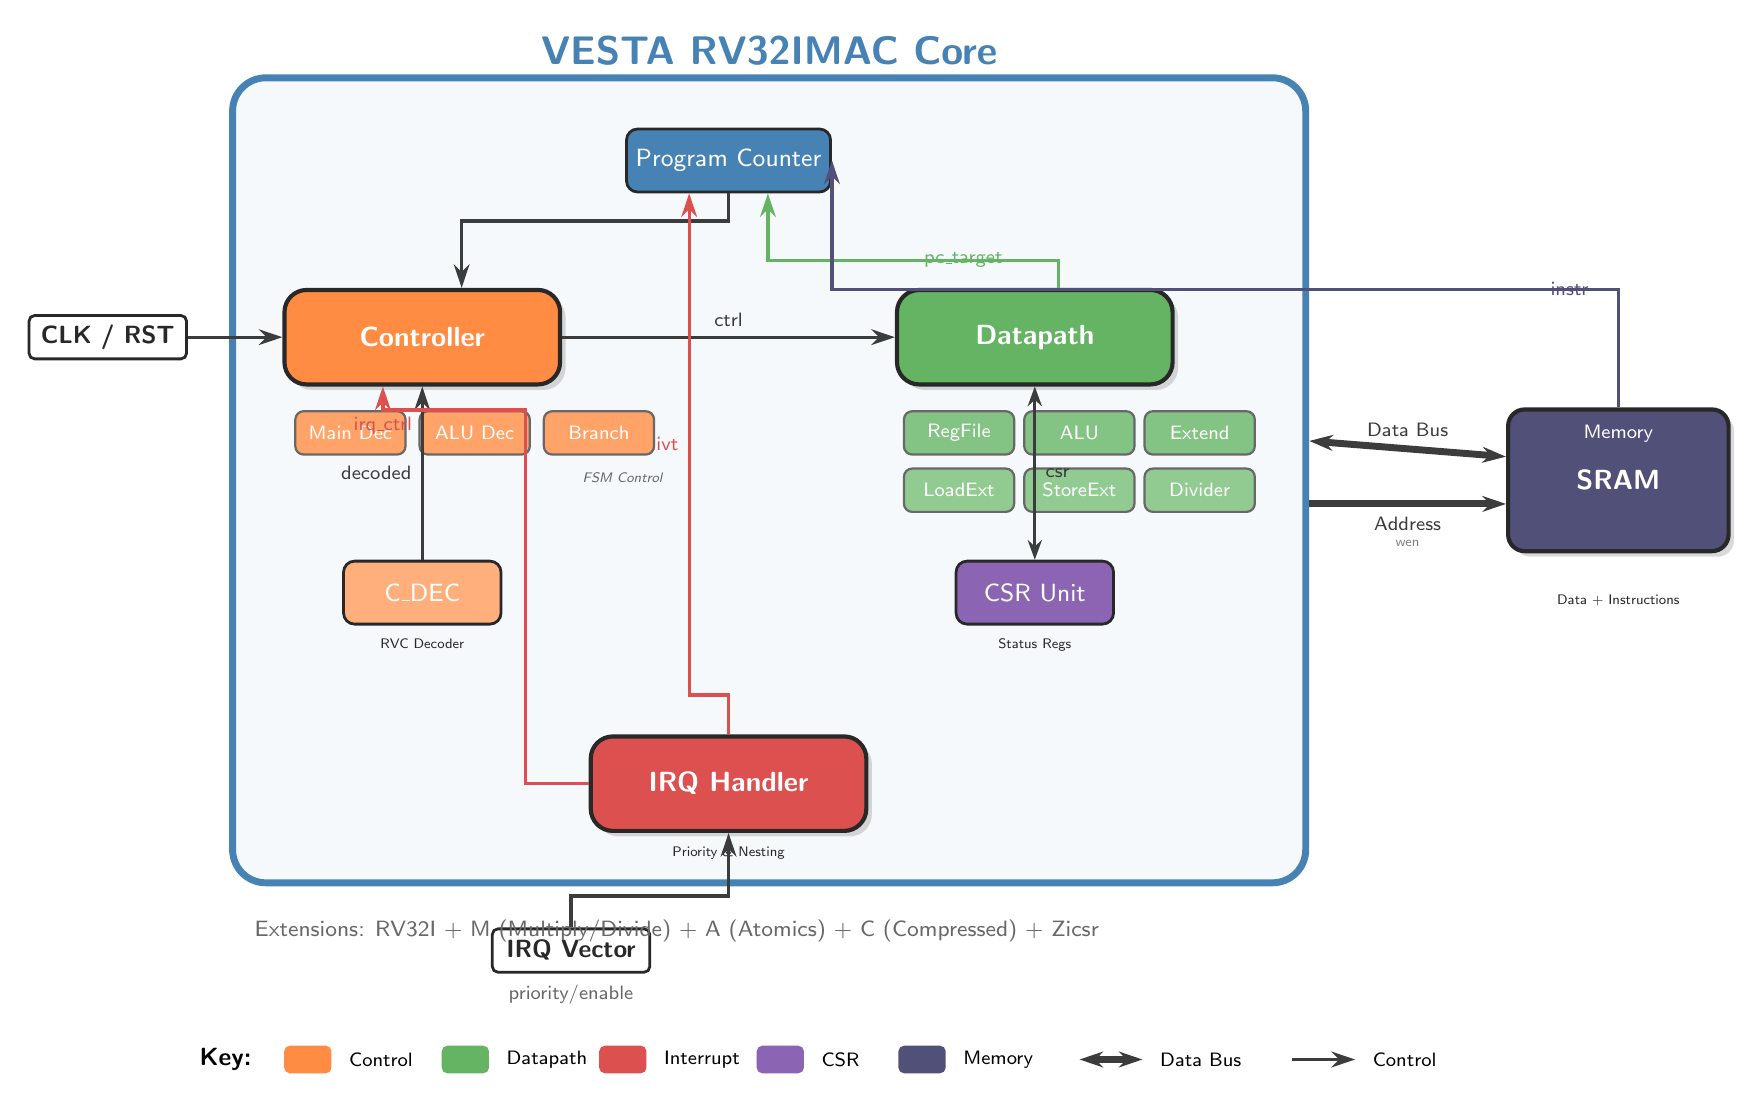
\begin{tikzpicture}[node distance=1.2cm and 1.5cm]

%===============================================================================
% VESTA CPU CORE CONTAINER
%===============================================================================
\begin{scope}[local bounding box=vestacore]

    %===========================================================================
    % PROGRAM COUNTER (Top center)
    %===========================================================================
    \node[subblock, fill=cpuCore] (pc) {Program Counter};

    %===========================================================================
    % CONTROLLER UNIT (Left, below PC)
    %===========================================================================
    \node[mainblock, fill=controlUnit, below left=1.2cm and 0.8cm of pc] (controller) {Controller};
    
    % Controller subblocks
    \node[tinyblock, fill=controlUnit!80, below=0.3cm of controller.south west, anchor=north west, xshift=0.15cm] (maindec) {Main Dec};
    \node[tinyblock, fill=controlUnit!80, right=0.15cm of maindec] (aludec) {ALU Dec};
    \node[tinyblock, fill=controlUnit!80, right=0.15cm of aludec] (brvalid) {Branch};
    
    %===========================================================================
    % DATAPATH UNIT (Right, below PC)
    %===========================================================================
    \node[mainblock, fill=dataUnit, below right=1.2cm and 0.8cm of pc] (datapath) {Datapath};
    
    % Datapath subblocks - arranged in 2 rows
    \node[tinyblock, fill=dataUnit!80, below=0.3cm of datapath.south west, anchor=north west, xshift=0.1cm] (regfile) {RegFile};
    \node[tinyblock, fill=dataUnit!80, right=0.1cm of regfile] (alu) {ALU};
    \node[tinyblock, fill=dataUnit!80, right=0.1cm of alu] (extend) {Extend};
    
    \node[tinyblock, fill=dataUnit!70, below=0.15cm of regfile.south west, anchor=north west] (loadext) {LoadExt};
    \node[tinyblock, fill=dataUnit!70, right=0.1cm of loadext] (storeext) {StoreExt};
    \node[tinyblock, fill=dataUnit!70, right=0.1cm of storeext] (div) {Divider};
    
    %===========================================================================
    % COMPRESSED INSTRUCTION DECODER (Below Controller)
    %===========================================================================
    \node[subblock, fill=controlUnit!70, below=2.2cm of controller] (cdec) {C\_DEC};
    \node[font=\tiny\sffamily, below=0.05cm of cdec, text=borderDark] {RVC Decoder};
    
    %===========================================================================
    % CSR UNIT (Below Datapath)
    %===========================================================================
    \node[subblock, fill=memoryUnit, below=2.2cm of datapath] (csr) {CSR Unit};
    \node[font=\tiny\sffamily, below=0.05cm of csr, text=borderDark] {Status Regs};
    
    %===========================================================================
    % IRQ HANDLER (Bottom center)
    %===========================================================================
    \node[mainblock, fill=irqUnit, below=1.8cm of $(cdec)!0.5!(csr)$] (irq) {IRQ Handler};
    \node[font=\tiny\sffamily, below=0.05cm of irq, text=borderDark] {Priority \& Nesting};
    
    %===========================================================================
    % STATE MACHINE indicator (in controller area)
    %===========================================================================
    \node[font=\tiny\sffamily\itshape, text=borderDark!70, below=0.1cm of brvalid, xshift=0.3cm] {FSM Control};

\end{scope}

%===============================================================================
% VESTA CORE BOUNDARY BOX
%===============================================================================
\begin{scope}[on background layer]
    \node[containerbox, fit=(pc)(controller)(datapath)(cdec)(csr)(irq)(maindec)(loadext)(div), 
          inner sep=18pt] (vestaborder) {};
\end{scope}

% Core label
\node[font=\Large\bfseries\sffamily, text=cpuCore, anchor=south] 
    at (vestaborder.north) {VESTA RV32IMAC Core};

%===============================================================================
% SRAM (External, Right side)
%===============================================================================
\node[memblock, fill=sramColor, right=2.5cm of vestaborder.east, anchor=west] (sram) {SRAM};
\node[font=\scriptsize\sffamily, text=textLight, below=0.1cm of sram.north] {Memory};
\node[font=\tiny\sffamily, below=0.4cm of sram, text=borderDark] {Data + Instructions};

%===============================================================================
% EXTERNAL INTERFACES
%===============================================================================

% IRQ Input (Bottom-left)
\node[ioport, below=1.2cm of irq, xshift=-2cm] (irqin) {IRQ Vector};
\node[font=\scriptsize\sffamily, below=0.02cm of irqin, text=borderDark!70] {priority/enable};

% Clock/Reset (Left side)
\node[ioport, left=1.2cm of controller] (clkrst) {CLK / RST};

%===============================================================================
% INTERNAL SIGNAL CONNECTIONS (Cleaned up routing)
%===============================================================================

% Controller to Datapath (control signals) - horizontal, no crossing
\draw[signal] (controller.east) -- (datapath.west)
    node[midway, above, font=\scriptsize\sffamily] {ctrl};

% PC to Controller (opcode/funct fields)
\draw[signal] (pc.south) -- ++(0,-0.35) -| ($(controller.north)+(0.5,0)$);

% Datapath to PC (branch target) - clean vertical then horizontal
\draw[signal, color=dataUnit] ($(datapath.north)+(0.3,0)$) -- ++(0,0.35) -| ($(pc.south)+(0.5,0)$)
    node[pos=0.25, right, font=\scriptsize\sffamily] {pc\_target};

% C_DEC to Controller - vertical connection, no crossing
\draw[signal] (cdec.north) -- (controller.south)
    node[midway, left, font=\scriptsize\sffamily] {decoded};

% CSR to Datapath - vertical connection
\draw[bidirectional] (csr.north) -- (datapath.south)
    node[midway, right, font=\scriptsize\sffamily] {csr};

% IRQ Handler to Controller - route left side to avoid crossings
\draw[signal, color=irqUnit] (irq.west) -- ++(-0.8,0) |- ($(controller.south)+(-0.5,-0.3)$) -- ($(controller.south)+(-0.5,0)$)
    node[pos=0.15, below, font=\scriptsize\sffamily] {irq\_ctrl};

% IRQ Handler to PC (ivt_entry) - route through center
\draw[signal, color=irqUnit] (irq.north) -- ++(0,0.5) -| ($(pc.south)+(-0.5,0)$)
    node[pos=0.75, left, font=\scriptsize\sffamily] {ivt};

% External IRQ input
\draw[signal] (irqin.north) -- ++(0,0.4) -| (irq.south);

% Clock/Reset to Controller
\draw[signal] (clkrst.east) -- (controller.west);

%===============================================================================
% MEMORY BUS CONNECTIONS (to SRAM)
%===============================================================================

% Main data bus from Datapath to SRAM
\draw[databidirectional] ($(vestaborder.east)+(0,0.5)$) -- ($(sram.west)+(0,0.3)$)
    node[midway, above, font=\scriptsize\sffamily] {Data Bus};

% Address bus
\draw[bussignal] ($(vestaborder.east)+(0,-0.3)$) -- ($(sram.west)+(0,-0.3)$)
    node[midway, below, font=\scriptsize\sffamily] {Address};

% Instruction fetch path (from SRAM back to PC/C_DEC)
\draw[signal, color=sramColor] (sram.north) -- ++(0,1.5) -| (pc.east)
    node[pos=0.05, right, font=\scriptsize\sffamily] {instr};

% Write enable
\node[font=\tiny\sffamily, text=borderDark!60] at ($(vestaborder.east)!0.5!(sram.west)+(0,-0.8)$) {wen};

%===============================================================================
% LEGEND
%===============================================================================
\begin{scope}[shift={($(vestaborder.south west)+(-0.5,-2.2)$)}]
    \node[font=\small\bfseries\sffamily, anchor=west] at (0,0) {Key:};
    
    \node[rectangle, fill=controlUnit, rounded corners=2pt, minimum width=0.6cm, minimum height=0.35cm] at (1.5,0) {};
    \node[font=\scriptsize\sffamily, anchor=west] at (1.9,0) {Control};
    
    \node[rectangle, fill=dataUnit, rounded corners=2pt, minimum width=0.6cm, minimum height=0.35cm] at (3.5,0) {};
    \node[font=\scriptsize\sffamily, anchor=west] at (3.9,0) {Datapath};
    
    \node[rectangle, fill=irqUnit, rounded corners=2pt, minimum width=0.6cm, minimum height=0.35cm] at (5.5,0) {};
    \node[font=\scriptsize\sffamily, anchor=west] at (5.9,0) {Interrupt};
    
    \node[rectangle, fill=memoryUnit, rounded corners=2pt, minimum width=0.6cm, minimum height=0.35cm] at (7.5,0) {};
    \node[font=\scriptsize\sffamily, anchor=west] at (7.9,0) {CSR};
    
    \node[rectangle, fill=sramColor, rounded corners=2pt, minimum width=0.6cm, minimum height=0.35cm] at (9.3,0) {};
    \node[font=\scriptsize\sffamily, anchor=west] at (9.7,0) {Memory};
    
    \draw[databidirectional] (11.3,0) -- ++(0.8,0);
    \node[font=\scriptsize\sffamily, anchor=west] at (12.2,0) {Data Bus};
    
    \draw[signal] (14,0) -- ++(0.8,0);
    \node[font=\scriptsize\sffamily, anchor=west] at (14.9,0) {Control};
\end{scope}

%===============================================================================
% ISA EXTENSIONS LABEL
%===============================================================================
\node[font=\footnotesize\sffamily, text=borderDark!70, anchor=north west] 
    at ($(vestaborder.south west)+(0.2,-0.3)$) 
    {Extensions: RV32I + M (Multiply/Divide) + A (Atomics) + C (Compressed) + Zicsr};

\end{tikzpicture}
\end{document}
